\documentclass{standalone}

\usepackage{tikz}
\usepackage{standalone}
\usepackage{color}
\usetikzlibrary{calc}
\usepackage{pgfplots}
\usetikzlibrary{shapes.multipart}

\begin{document}

    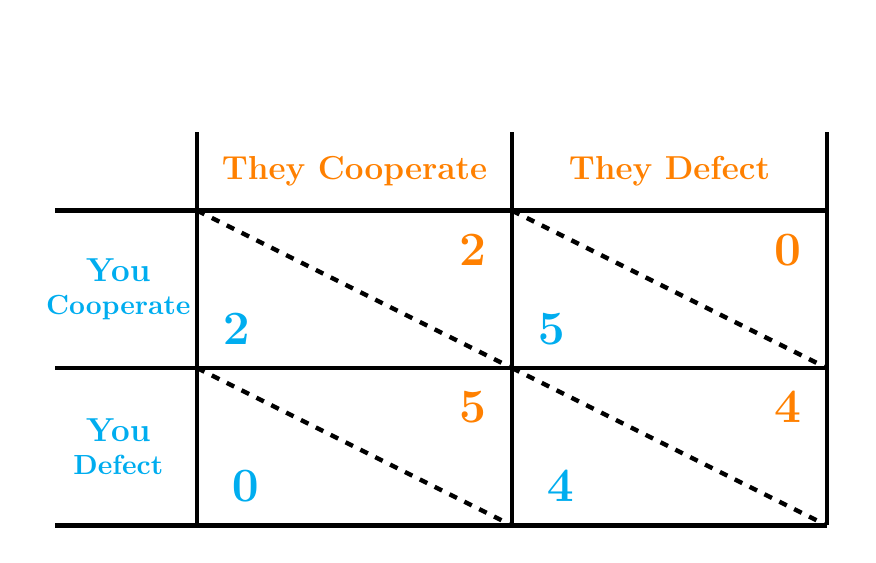
\begin{tikzpicture}
    \tikzstyle{state}=[minimum width=1cm, font=\boldmath];

    % horizontal lines
    \draw[-, line width=2pt, ultra thick] (-1.8, -2) -- (8, -2) node[right] {};
    \draw[-, line width=2pt, ultra thick] (-1.8, 0) -- (8, 0) node[right] {};
    \draw[-, line width=2pt, ultra thick] (-1.8, 2) -- (8, 2) node[right] {};

    % vertical lines
    \draw[-, line width=2pt, ultra thick] (0,-2) -- (0,3) node[above] {};
    \draw[-, line width=2pt, ultra thick] (4,-2) -- (4,3) node[above] {};
    \draw[-, line width=2pt, ultra thick] (8,-2) -- (8,3) node[above] {};

    % dashed lines
    \draw[dashed, line width=1pt, ultra thick] (0, 2) -- (4, 0) node[right] {};
    \draw[dashed, line width=1pt, ultra thick] (4, 2) -- (8, 0) node[right] {};
    \draw[dashed, line width=1pt, ultra thick] (0, 0) -- (4, -2) node[right] {};
    \draw[dashed, line width=1pt, ultra thick] (4, 0) -- (8, -2) node[right] {};

    % player's actions
    \node[circle, ultra thick] (0) at (2, 2.5) [state] {\large \textbf{\textcolor{orange}{They Cooperate}}};
    \node[circle, ultra thick] (0) at (6, 2.5) [state] {\large \textbf{\textcolor{orange}{They Defect}}};
    \node[circle, ultra thick] (0) at (-1, 1) [state, align=center] {\large \textbf{\textcolor{cyan}{You}} \\
    \textbf{\textcolor{cyan}{Cooperate}}};
    \node[circle, ultra thick] (0) at (-1, -1) [state, align=center] {\large \textbf{\textcolor{cyan}{You}} \\
    \textbf{\textcolor{cyan}{Defect}}};
    \node[circle, ultra thick] (0) at (3.5, 1.5) [state] {\LARGE \textbf{\textcolor{orange}2}};
    \node[circle, ultra thick] (0) at (3.5, -0.5) [state] {\LARGE \textbf{\textcolor{orange}5}};
    \node[circle, ultra thick] (0) at (0.5, 0.5) [state] {\LARGE \textbf{\textcolor{cyan}2}};
    \node[circle, ultra thick] (0) at (0.5, -1.5) [state] {\LARGE\textbf{ \textcolor{cyan}0}};
    \node[circle, ultra thick] (0) at (7.5, 1.5) [state] {\LARGE \textbf{\textcolor{orange}0}};
    \node[circle, ultra thick] (0) at (7.5, -0.5) [state] {\LARGE \textbf{\textcolor{orange}4}};
    \node[circle, ultra thick] (0) at (4.5, 0.5) [state] {\LARGE \textbf{\textcolor{cyan}5}};
    \node[circle, ultra thick] (0) at (4.5, -1.5) [state] {\LARGE\textbf{ \textcolor{cyan}4}};

    \end{tikzpicture}

\end{document}